\documentclass[tikz,border=2pt]{standalone}
\usepackage{amsmath,amssymb}
\usetikzlibrary{arrows.meta}
\begin{document}
% Varying annuity-due paying 1 at time 0 and 2 at time 1 if alive, v = 0.95, p_x = 0.9:
% Y = 2.9 with probability 0.9 and Y = 1 with probability 0.1, so E[Y] = 2.71 and Var(Y) = (1.9)^2(0.9)(0.1) = 0.3249.
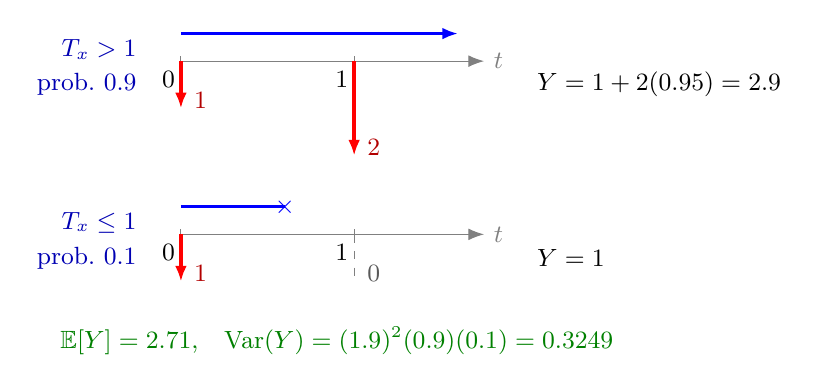
\begin{tikzpicture}[font=\small, >={Latex[length=2mm]}, x=2.2cm]
  \newcommand{\taxis}{%
    \draw[gray, ->] (0,0) -- (1.75,0) node[right] {$t$};
    \foreach \t in {0,1} \draw[gray] (\t,-0.07) -- (\t,0.07);
    \node[anchor=north east, inner sep=2pt] at (0,-0.05) {$0$};
    \node[anchor=north east, inner sep=2pt] at (1,-0.05) {$1$};}
  % survives to time 1
  \taxis
  \draw[blue, very thick, ->] (0,0.35) -- (1.6,0.35);
  \node[blue!70!black, anchor=east] at (-0.2,0.15) {$T_x>1$};
  \node[blue!70!black, anchor=east] at (-0.2,-0.3) {prob.\ $0.9$};
  \draw[red, very thick, ->] (0,0) -- (0,-0.6);
  \node[red!70!black, anchor=west] at (0.02,-0.5) {$1$};
  \draw[red, very thick, ->] (1,0) -- (1,-1.2);
  \node[red!70!black, anchor=west] at (1.02,-1.1) {$2$};
  \node[anchor=west] at (2.0,-0.3) {$Y=1+2(0.95)=2.9$};
  % dies before time 1
  \begin{scope}[yshift=-2.2cm]
    \taxis
    \draw[blue, very thick] (0,0.35) -- (0.6,0.35);
    \node[blue] at (0.6,0.35) {$\times$};
    \node[blue!70!black, anchor=east] at (-0.2,0.15) {$T_x\le1$};
    \node[blue!70!black, anchor=east] at (-0.2,-0.3) {prob.\ $0.1$};
    \draw[red, very thick, ->] (0,0) -- (0,-0.6);
    \node[red!70!black, anchor=west] at (0.02,-0.5) {$1$};
    \draw[gray, dashed] (1,0) -- (1,-0.6);
    \node[gray!70!black, anchor=west] at (1.02,-0.5) {$0$};
    \node[anchor=west] at (2.0,-0.3) {$Y=1$};
  \end{scope}
  \node[green!50!black, anchor=north] at (0.9,-3.25) {$\mathbb E[Y]=2.71$,\quad $\operatorname{Var}(Y)=(1.9)^2(0.9)(0.1)=0.3249$};
\end{tikzpicture}
\end{document}
